\documentclass[12pt]{article}

\usepackage{amsmath}
\usepackage[dvips]{graphicx}
\usepackage{verbatim}

\title{Stat 4201 HOMEWORK 2}
\author{Mengqi Zong $<mz2326@columbia.edu>$}

\begin{document}

\maketitle

\section{Problem Set 2}

\begin{enumerate}
\item Consider the RatPupWeight (the weight of rat pups) in R library nlme:\\
data(RatPupWeight,package="nlme")

\begin{enumerate}
\item Disregarding the effects of all the other variables, determine
  whether there is a significant difference between mean weight of rat
  pubs in the control and active (low/high combined) treatment groups
  using each of the following procedures:
  
  \begin{itemize}
    \item A parametric procedure
    \item A non-parametric procedure
    \item A re-sampling procedure
  \end{itemize}

\item Discuss the assumption underlying the analysis in (1) above,
  their validity, and any remedial measures to be taken..
\item Determine whether there is a significant association between
  weight and Litter Size for each of the following:

  \begin{itemize}
    \item A parametric procedure
    \item A non-parametric procedure
  \end{itemize}

\end{enumerate}
\end{enumerate}

\section{Answers to Problem 1}


\begin{enumerate}
\item Problem 1.1
  \begin{enumerate}
  \item A parametric procedure\\
    I use two-sample t-test to do the data analysis. And the
    result from R is as follow:

\begin{verbatim}
	Two Sample t-test

data:  active$weight and control$weight 
t = -5.8809, df = 320, p-value = 1.027e-08
alternative hypothesis: true difference in means is not equal to 0 
95 percent confidence interval:
 -0.5484473 -0.2734790 
sample estimates:
mean of x mean of y 
 5.913770  6.324733 

\end{verbatim}

    We can see that two-sample t-test indicates that the two groups'
    mean weight of rat pubs are significantly different.

  \item A non-parametric procedure\\
    I use Wilcoxon rank sum test with to do the data analysis. And
    the result from R is as follow:

\begin{verbatim}

	Wilcoxon rank sum test with continuity correction

data:  active$weight and control$weight 
W = 7628, p-value = 2.696e-09
alternative hypothesis: true location shift is not equal to 0 

\end{verbatim}

    From Wilcoxon rank sum test, we can see that there is a
    significant difference between mean weight of rat pubs.

  \item A re-sampling procedure\\
    I use bootstrap to do the data analysis.
    Using bootstrap to calculate the $Weight_{control}-
    Weight_{active}$, I get the $95\%$ confidence interval: 
    $ [0.2706, 0.5649] $. Apparently, 0 is not in the confidence
    interval, and there is a significant difference between mean
    weight of rat pubs.

  \end{enumerate}

\item Problem 1.2\\
  \begin{enumerate}
  \item Two-sample t-Test\\
    About t-test, its assumptions are independent and
    normality.
    
    As to independent, since the data is about every rat pup's
    weight, logically, there is no obvious dependency among rat
    pups. So the data satisfy the requirement of independent.

    As to normality, I first use histogram to get a first look on
    the data. Control group's histogram is shown in
    Fig~/ref{fig:hisc}, Active group's histogram is shown in
    Fig~/ref{fig:hisa}. From the histogram, we can see that the two
    groups of data are basically normally distributed, only the
    active group is a little bit heavy-tailed.

    \begin{figure}[ht!]
      \centering
      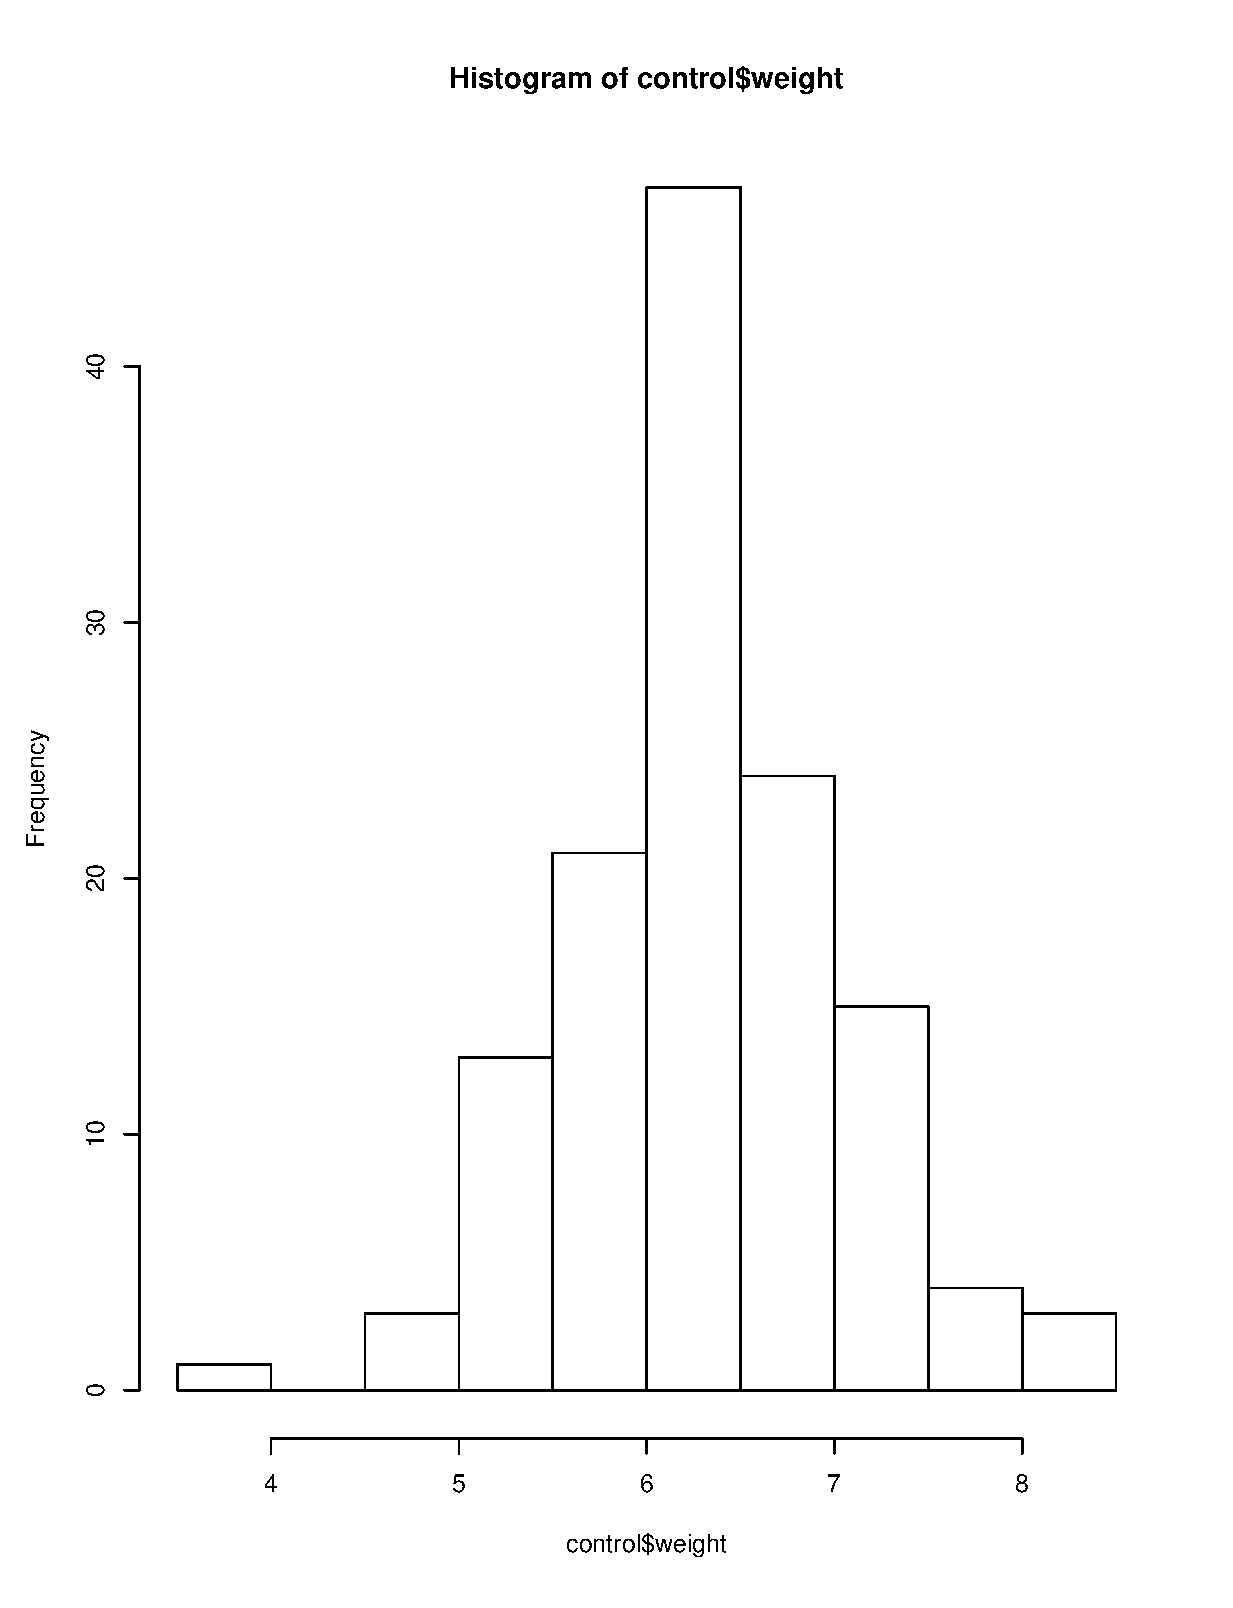
\includegraphics[width=0.7\textwidth]{hist_control}
      \caption{Weight of rat pups from control group \label{fig:histc}}
    \end{figure}

    \begin{figure}[ht!]
      \centering
      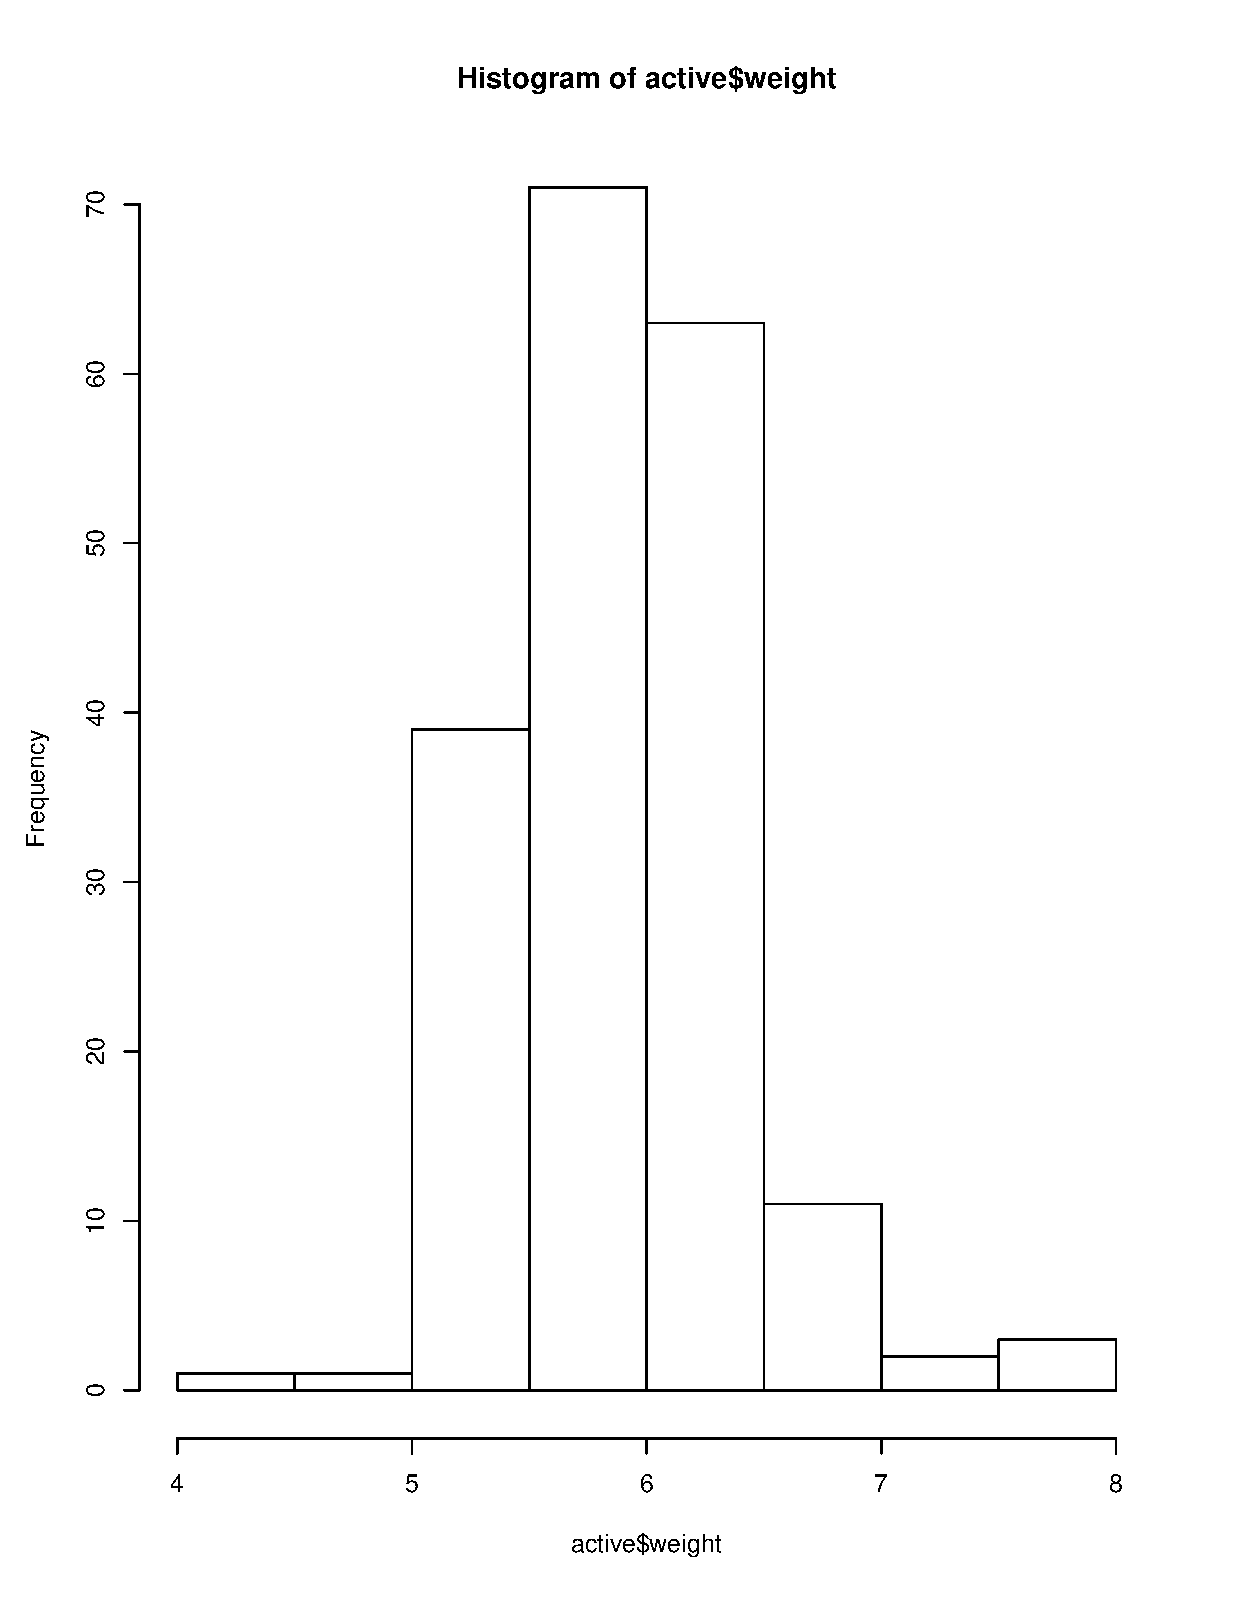
\includegraphics[width=0.7\textwidth]{hist_active}
      \caption{Weight of rat pups from active group \label{fig:hista}}
    \end{figure}

    Then, I use Shapiro-Wilk normality test to get further
    information. And the two groups result from R are as follow:

\begin{verbatim}

	Shapiro-Wilk normality test

data:  control$weight 
W = 0.9847, p-value = 0.1502

	Shapiro-Wilk normality test

data:  active$weight 
W = 0.969, p-value = 0.00031

\end{verbatim}

    From the Shapiro-Wilk normality test, we can see that data from
    control group is approximately normally distributed
    ($ p-value_{control}  = 0.1502 > 0.1 $). However, data from active
    group is not normally distributed ($ p-value_{active}  = 0.00031 <
    0.1 $). From the histogram, we can easily see that active group is
    heavily-tailed. 

    In total, I think this does not affect our two-sample t-test
    very much. First, it is reasonable that active group's is not
    normally distributed. Because data in active group are from two
    different treatment group: low and high. And it is quite clear
    that different treatment makes the weight quite
    different. Second, t-test is relatively robust against normality
    and differing standard deviations. Both group has more than 100
    examples ($n_{active} = 191, n_{control} = 131 $) and their sizes
    are not quite different ($n_{active} / n_{control} = 1.46 $). Also,
    there variance are quite similar ($\sigma_{active} /
    \sigma_{control} = 0.47 $), and most of the difference in
    variance is probably due to their different size. In all,
    the result from the t-test is reasonable valid.

  \item Wilcoxon rank sum test\\
    About Wilcoxon rank sum test, a very general formulation is to
    assume that (from Wikipedia):
    \begin{enumerate}
      \item All the observations from both groups are independent of
        each other.
      \item The respnse are ordinal.
    \end{enumerate}
    As I showed before, independent is satisfied. As to ordinal, it
    is easily satisfied. So Wilcoxon rank sum test is valid for the
    data.

  \item Bootstrap test\\
    Bootstrap assumes normality and independent, same as two-sample
    t-test. This has been discussed before.

  \end{enumerate}

\item Problem 1.3
  \begin{enumerate}
  \item A parametric procedure\\
    I use Pearson's product-moment correlation coefficient to test the
    association. And here is the result from R:

\begin{verbatim}

	Pearson's product-moment correlation

data:  mix$weight and mix$Lsize 
t = -6.9704, df = 320, p-value = 1.813e-11
alternative hypothesis: true correlation is not equal to 0 
95 percent confidence interval:
 -0.4543363 -0.2642549 
sample estimates:
       cor 
-0.3630671 

\end{verbatim}
 
    From the Pearson's product-moment correlation, we can see that
    there is a significant correlation between weight and Litter
    Size.
  \item A non-parametric procedure\\
    I use Spearman's rank correlation coefficient to test the
    association. Here is the result from R:

\begin{verbatim}

	Spearman's rank correlation rho

data:  mix$weight and mix$Lsize 
S = 7204569, p-value = 7.074e-08
alternative hypothesis: true rho is not equal to 0 
sample estimates:
       rho 
-0.2947795 

\end{verbatim}

    From the Spearman's rank correlation coefficient, we can see that
    there is a significant correlation between weight and Litter Size.

  \end{enumerate}

\end{enumerate}

\section{Answers to Problem 2}
 
Sorry, as a CS major, it's quite hard for me to learn that much in
just one week. I don't have time to do this question :/

\section{Appendix}
The code is listed below:

\verbatiminput{hmwk2.r}

\end{document}